\chapter{Data Aggregation and Modeling}   \label{ch:data-aggregation}
\graphicspath{{Part1/Chapter1/figures/}}

Along with the advent of Web 2.0, a substantial amount of high-demand information continue to be created and expanded over multiple social services. In particular, information about events, illustrative media and participants' connections are in constant growth. However, this information is often incomplete and locked into the sites, providing limited event coverage and no interoperability of the description. Integrating these distributed data sources into one unified platform is a key factor to enable rich presentation and search of all event content. One major concern that rises in this context is how to ensure a flexible integration that aggregates incrementally different sources of data. The goal is to achieve data integration in reasonable levels of effort and to face the dynamics of social services. In this chapter, we present our framework to integrate data ensuring a certain level of flexibility. Moreover, we explore the intrinsic connection between events and media based on explicit metadata.

\section{Data Aggregation}   \label{sec:data-scraping}
In this section, we overview the definition of a Web service. Then, we describe how data from event and media Web services has been collected and interlinked in a flexible way.

\subsection{Web Service Definition}	
Web Service has been defined by the W3C as ``a software system designed to support interoperable machine-to-machine interaction over a network.''~\cite{WS:2004}. It provides an application-programming interface (API) which describes a specification of remote request-response calls that could be consumed by other systems. In this context, a Web service is sometimes considered as a synonym of Web API. In Web 2.0, the most common API is based on REST architecture in which ``the primary purpose of the service is to manipulate XML representations of Web resources using a uniform set of \emph{stateless} operations''~\cite{WS:2004}. REST stands for Representational State Transfer, and it has emerged in the last few years as a predominant Web service design model. It is an alternative way to define Web services and has been introduced in 2000 in the doctoral dissertation of Roy Fielding, one of the principal authors of the HTTP specification. REST strictly refers to a collection of network architecture principles which outline how resources are defined, addressed and transferred over HTTP. With REST, each resource is referenced with a global identifier (e.g. URI in HTTP). To interact with a resource, an application needs to know the identifier of the resource, the action required and the format of the response. Most of existing Web APIs are currently based on REST architecture, and they define a set of HTTP request methods, along with associated responses usually serialized in XML and JSON formats.

\subsection{REST-based Scraper}	

Web services such as Eventful, Last.fm or YouTube become increasingly important for creating Web content mash-ups. Yet, collecting data from these heterogeneous platforms implies the studying of related API specifications which differ in terms of policy, HTTP methods and response schema. To alleviate this task, one typical solution is to design a unified interface that combines various APIs and manages some tasks such as policy management, requests chaining and merging response structures. Some tools providing this solution have been emerged with the aim to save developers' efforts. 

For instance, \textsc{API Blender}~\cite{Gouriten:WWW12} is an open-source that integrate five platforms, namely: Twitter, Facebook, Flickr, Google+ and YouTube. It describes a Web API using a set of JSON serialized objects including the definition of access policies and API methods. For example, the ``Policy'' object describes the number of requests per hour and the too-many-calls response code. Although \textsc{API Blender} supports a high flexibility to collect data, it does not address the difference between response schemata. Another tool is the media collector developed for \textsc{Media Finder} application~\cite{Rizzo:SAM12}. It enables a parallel key-search over a variety of social networks and exports results in a unified output. It is based on a common alignment response schema in order to be agnostic of a particular social network. The schema describes a set of metadata such as url, type (e.g. photo or video), message (e.g. description of media item), etc. However, there is no support for policy management and the response schema provides very basic information. 

In order to ensure a flexible data collection, there is a need for a unified interface that retrieves data from event and media Web services, and exploits the similarity between their Web APIs. We propose the framework\footnote{\url{http://eventmedia.eurecom.fr/scrap}} illustrated in Figure~\ref{fig:crawler-architecture} and composed of two main components: the Unified REST Module and the Scraping Processor, described as following.

\begin{figure}[htbp]
  \centering
  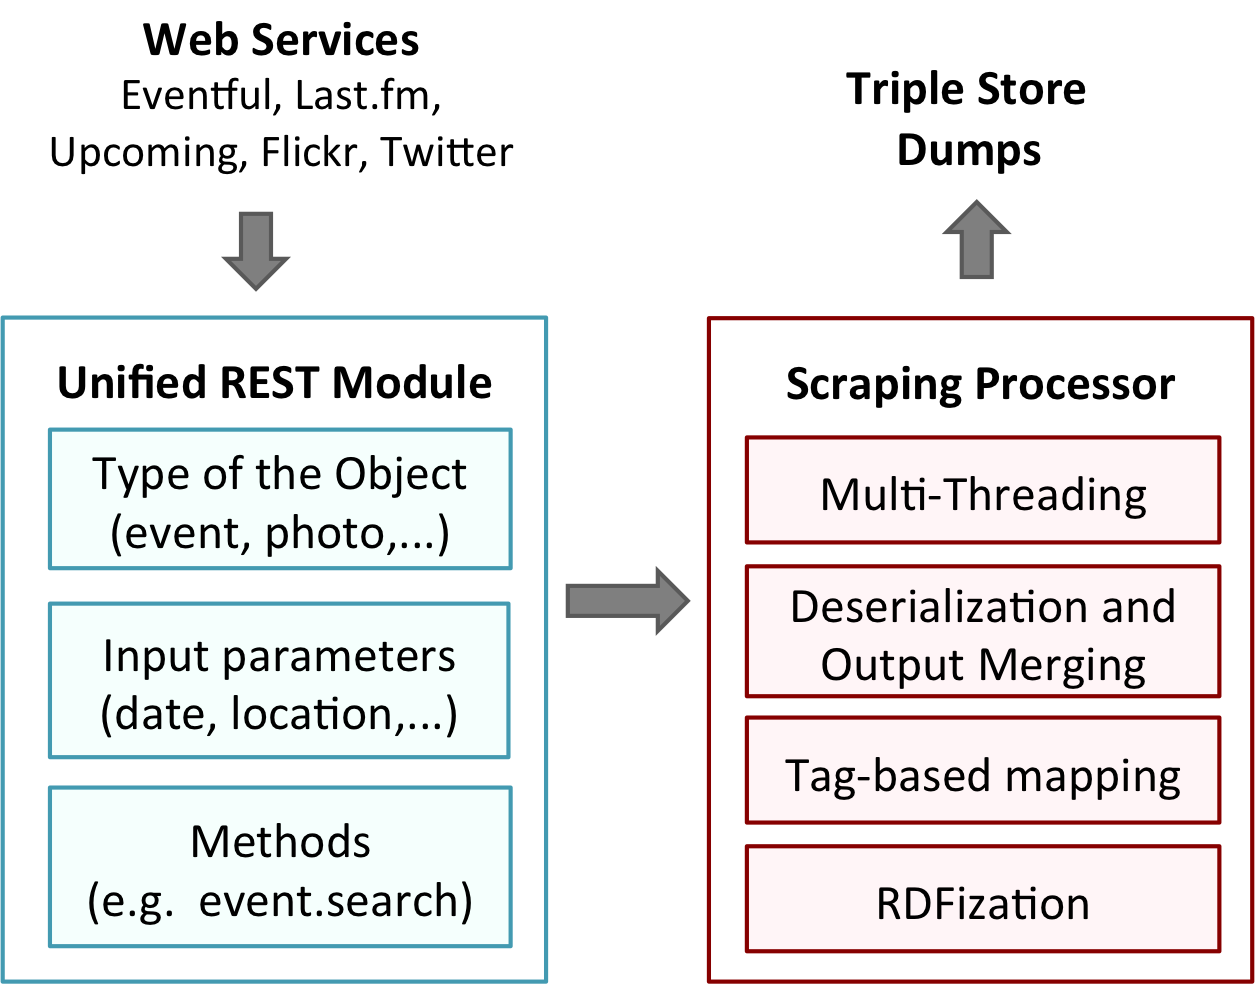
\includegraphics[scale=0.4]{crawler-architecture.png}
  \caption{Rest-based Scraper Architecture}
  \label{fig:crawler-architecture}
\end{figure}

\myparagraph{Unified REST Module} It is based on a RESTful service that allows unifying various Web APIs by exploiting their commonality in terms of HTTP methods, objects and input parameters. Each source API (e.g. Eventful API) is associated with a descriptor file serialized in JSON which provides useful information to handle REST requests. The descriptor file contains global parameters such as the API key, the API root path and a dictionary of URLs, as depicted in Listing~\ref{lst:DescFile}. In addition, the descriptor file contains an array of query objects. Each query object represents a mapping between our REST URL pattern and the source API URL pattern that describes a REST method and its input parameters. An example of a query object is depicted in Listing~\ref{lst:ObjectQuery}. 

\vspace{1mm}
\begin{lstlisting}[language=json,caption={Global parameters in Last.fm descriptor file},label={lst:DescFile}][H]
{
    "APIName": "Lastfm",
    "APIRootURL": "http://ws.audioscrobbler.com/2.0/?method=",
    "APIKey": "c650...",

    "Prefixes":{
                "publisher": "http://www.last.fm",
                "event": "http://www.last.fm/event/",
                "venue": "http://www.last.fm/venue/",
                "agent": "http://www.last.fm/music/"
            }
}	
\end{lstlisting}

In order to manage the requests chaining, each query object has a type which is used to retrieve the description of main elements (e.g. event, photo, video), and to perform sub-queries that fetch addition information (artist, attendee, etc.). We have defined our own REST methods to search for events, photos and videos, respectively. These methods have as input a set of parameters such as the original sources (e.g. last.fm, eventful, etc.) and other additional filters (e.g. category, location, date, etc.). Thus, the user can request in parallel multiple Web services by specifying the list of sources into one request. This RESTful service is flexible enough, so that new methods can be conveniently created and a new similar REST-inspired Web API can be simply integrated by adding the associated JSON descriptor file.

\vspace{1mm}
\begin{lstlisting}[language=json,caption={Query object for collecting events in Last.fm},label={lst:ObjectQuery}]
"Query": [
          {
            "Type": "events",
            "Method": "{0}geo.getevents&api_key={1}",
            "Inputs": [
                {
                   "Name": "Location",
                   "Format": "&location={0}",
                   "Required" : "true"
                },
                {
                   "Name": "LocationRadius",
                   "Format": "&lat={0}&long={1}&distance={2}",
                   "Required" : "true"
                },
                {
                   "Name": "PageNumber",
                   "Format": "&page={0}"
                },
                {
                   "Name": "PageSize",
                   "Format": "&limit={0}"
                }
            ]
          }
  ]	
\end{lstlisting}


\myparagraph{Scraping Processor} It is designed to manage requests and process data. It provides a scraping engine to enable multi-threading, where each new request is associated with a thread instance of scraping process. This engine allows only a limited number of thread processes in parallel to respect the Web APIs limits. Moreover, the Scraping Processor handles other tasks for processing data, starting from JSON de-serialization to RDF conversion and loading into a triple store. More precisely, data retrieved is de-serialized and exported into a common schema providing descriptions of a set of objects, namely; event, location, agent, user, photo and video. Then, we employ a tag-based mapping consuming some metadata in order to establish links between events and media (details in Section ~\ref{sec:explicit-linkage}). This framework is meant to ease the addition of new services for collecting events and media. It also offers other REST methods for monitoring tasks such as tracking or stopping the current scraping processes.  

\subsection{Explicit Linkage} \label{sec:explicit-linkage}

The explicit linkage of resources is straightforward in the presence of shared keys (ISBN, hashtag, etc). Thus, we explore the overlap in metadata that exists between some event and media services.

\begin{itemize}

\item Last.fm and Upcoming with Flickr: Explicit relationships between events and photos exist in Flickr using machine tags such as \texttt{lastfm:event=ID} where \texttt{ID} is the identifier of a specific event (Figure~\ref{fig:flickr-tag}). These tags are used as filters when searching for photos. Then, each photo resource is linked with the event resource that refers to it.

\begin{figure}[htbp]
  \centering
  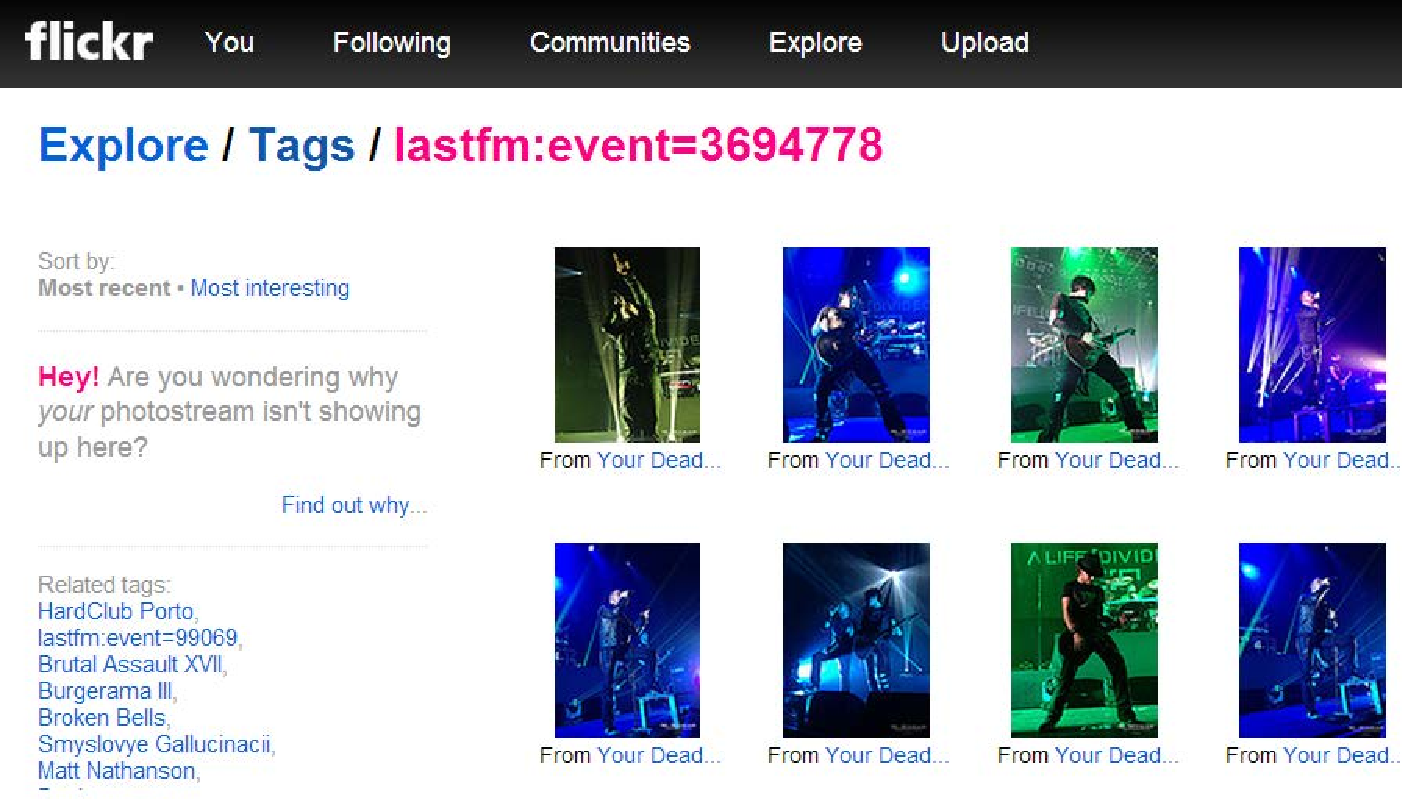
\includegraphics[scale=0.45]{flickr-tag.pdf}
  \caption{Photos with a machine tag identifying one Last.fm event}
  \label{fig:flickr-tag}
\end{figure}

\begin{figure}[htbp]
  \centering
  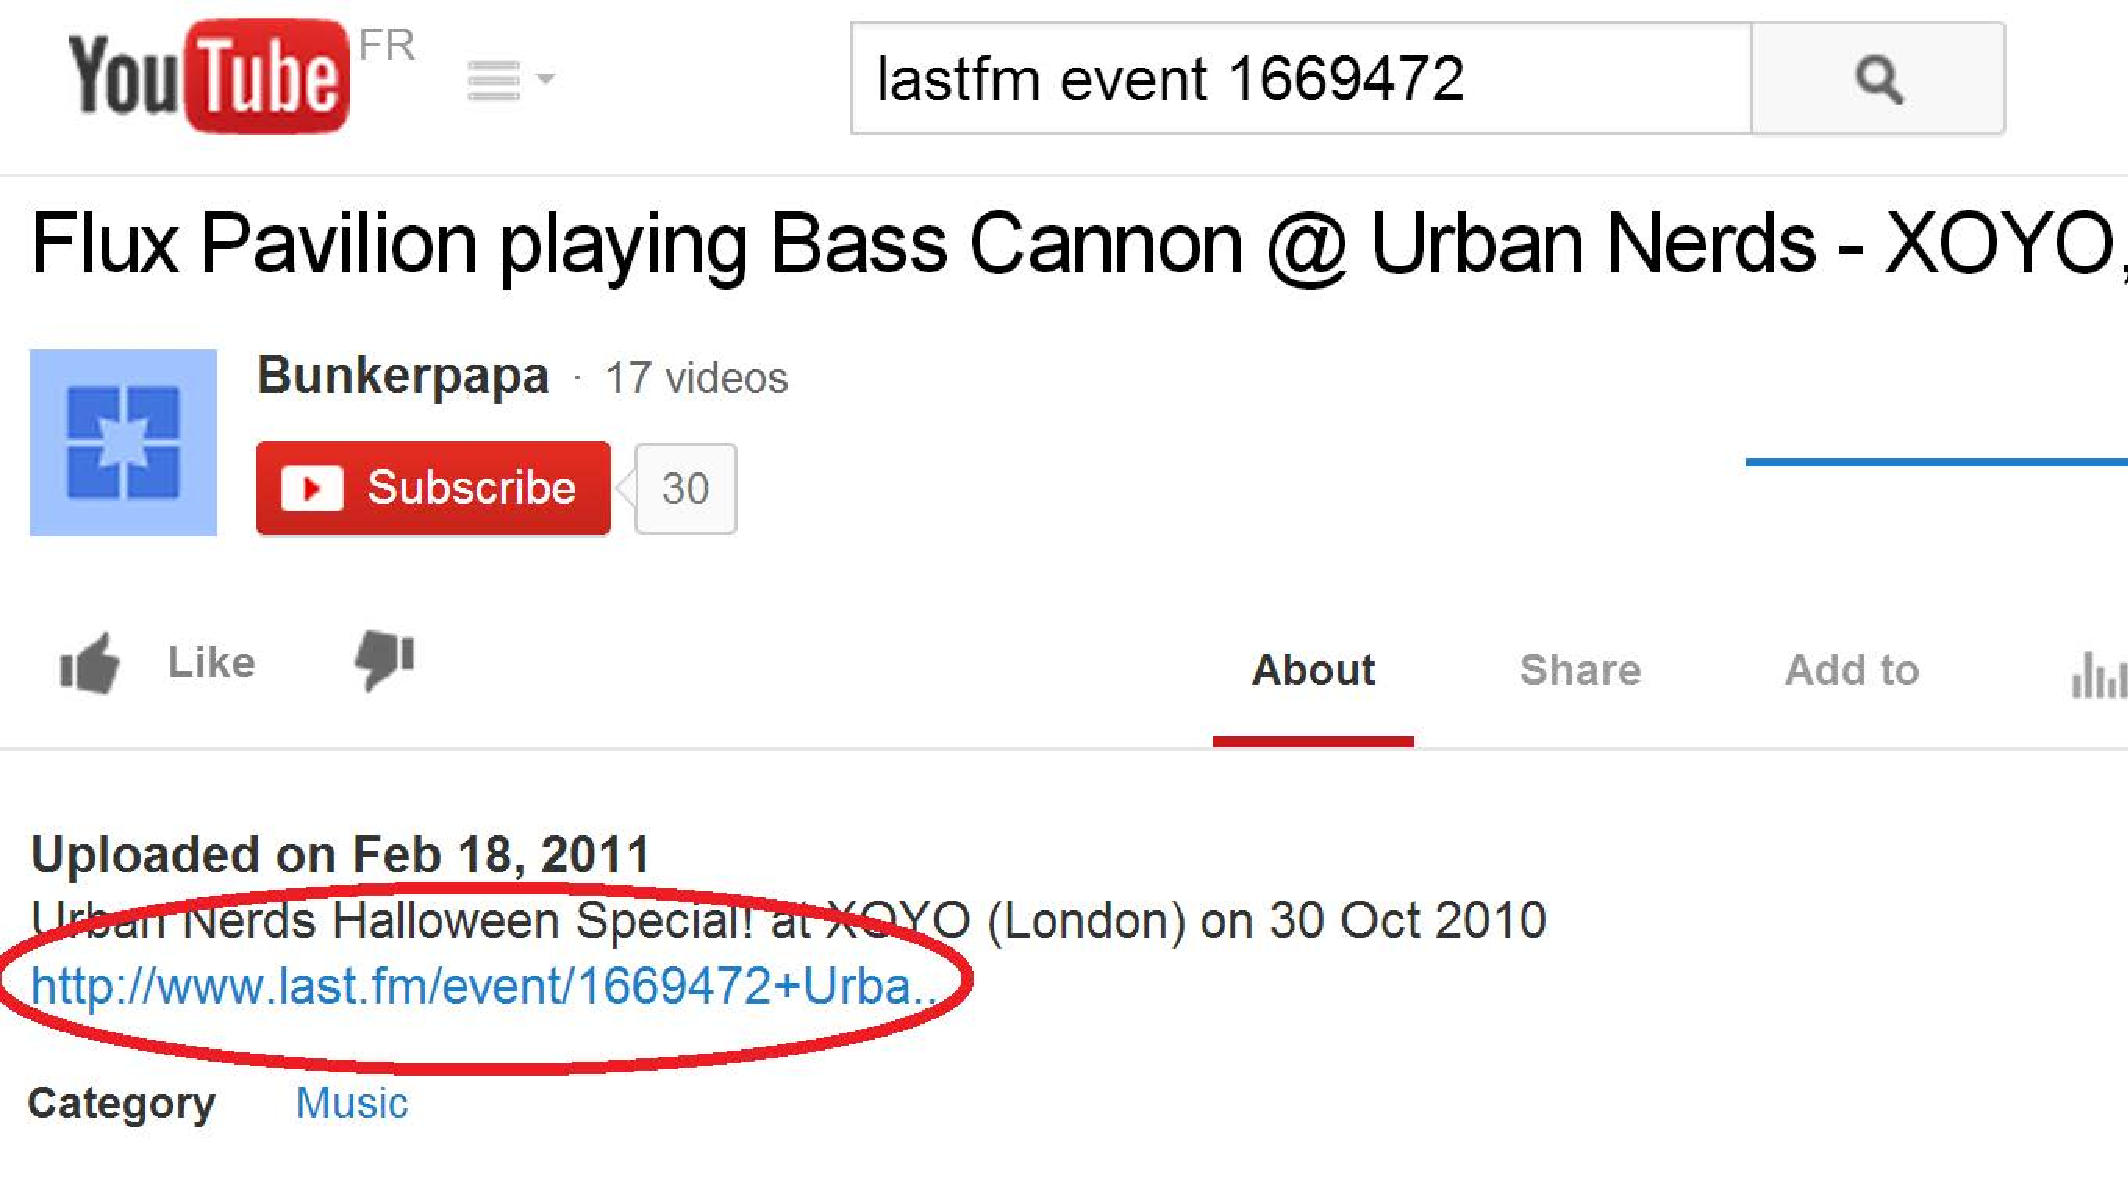
\includegraphics[scale=0.3]{youtube-tag.pdf}
  \caption{Video description including a Last.fm event URL}
  \label{fig:youtube-tag}
\end{figure}

\item Last.fm with YouTube: Similarly, some of YouTube videos have a description including a Last.fm event URL. Thus, videos can be retrieved by a simple keyword search such as ``lastfm event''. An event identifier could also be added when collecting videos for a specific event. Figure~\ref{fig:youtube-tag} illustrates an example of video that will be associated with the event resource identified by \emph{ID=1669472} in Last.fm. 

\item Lanyrd with Twitter: We also benefit from the overlap between Lanyrd and Twitter, where a hashtag associates each tweet with its related conference. These hashtags are provided by Lanyrd website as depicted in Figure~\ref{fig:lanyrd-tag}

\begin{figure}[H]
  \centering
  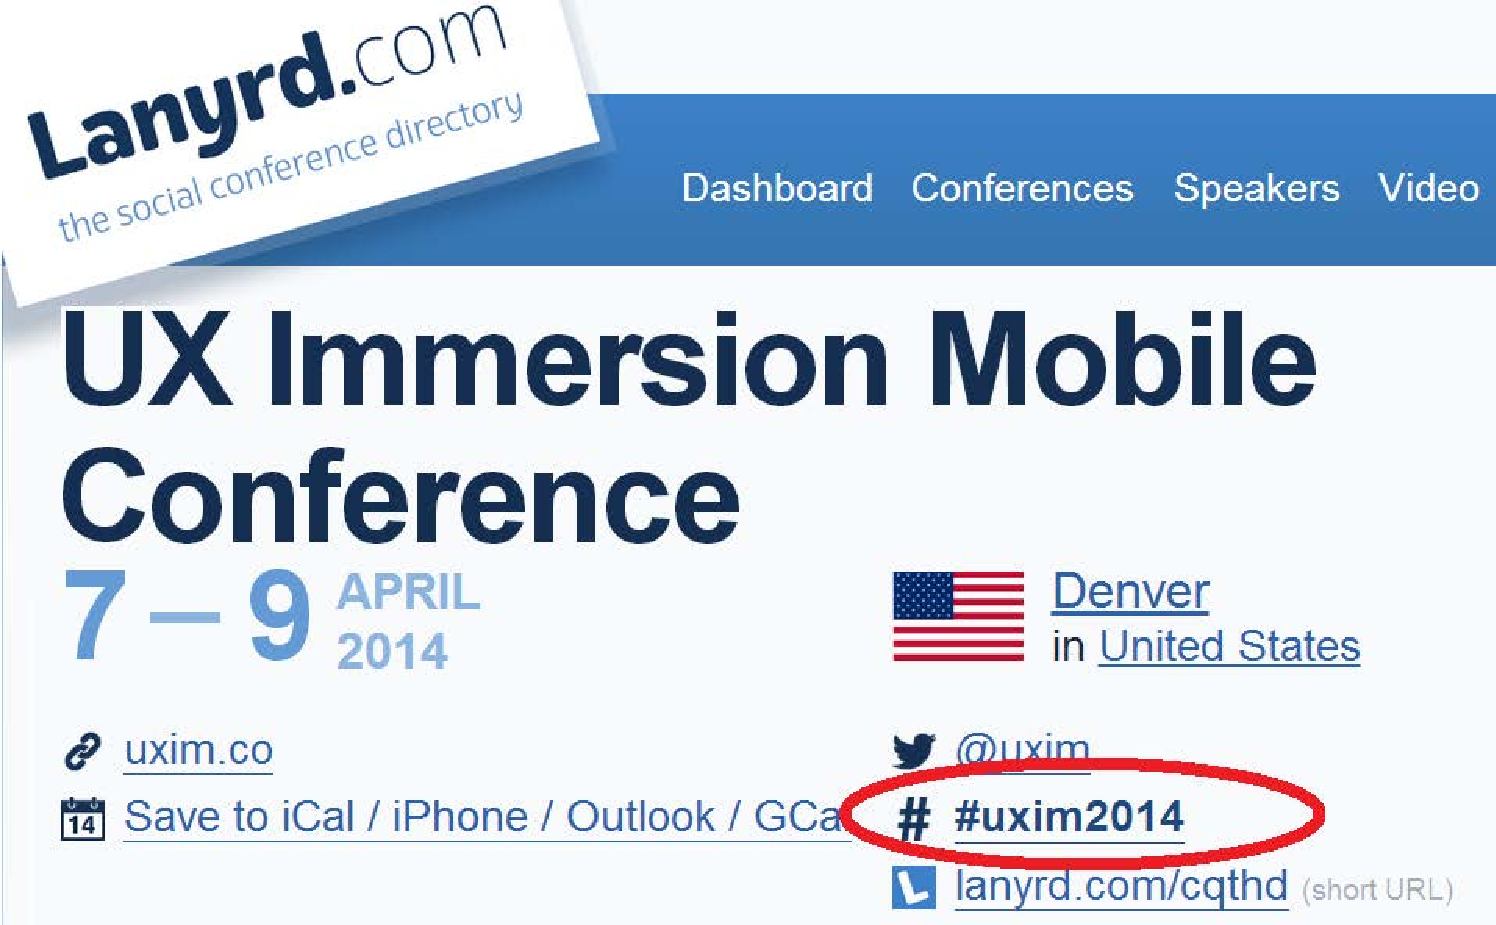
\includegraphics[scale=0.45]{lanyrd-tag.pdf}
  \caption{Lanyrd conference associated with the Twitter hashtag ``{\#}uxim2014''}
  \label{fig:lanyrd-tag}
\end{figure}

\end{itemize}

\subsection{Real-time Scraping}
New events are taking place everyday and people keep sharing an ever increasing amount of related media. Such evolution requires a real-time processing that retrieves fresh data and updates the triple store. To achieve this, we developed a live extractor which consumes the feeds provided by some Web services. More specifically, we use the Flickr feeds\footnote{\url{http://api.flickr.com/services/feeds/photos_public.gne?tags=*:event}}  including the tag ``*:event=''. Then, a scheduled process reads the feeds every 10 minutes, and trigger accordingly the scraping requests to retrieve the descriptions of events and photos.  On an average week, we observe 2000 new photos associated with 160 events (Figure~\ref{fig:flickr-rss}). Similarly, we also use the Lanyrd feeds\footnote{\url{http://api.lanyrd.com/conferences}} that provides fresh conference information including the main hashtag required to retrieve related tweets. 

\begin{figure}[H]
  \centering
  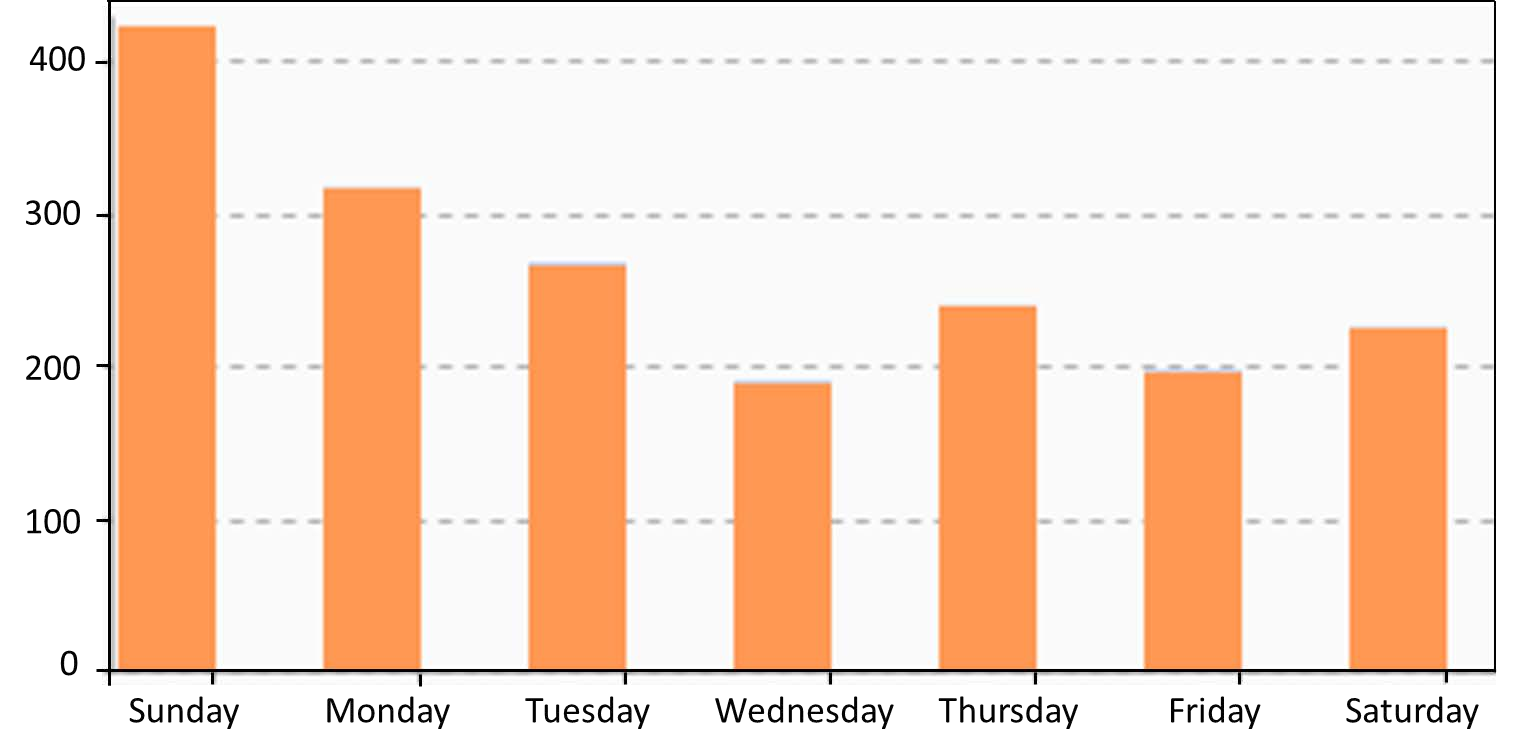
\includegraphics[scale=0.42]{rss-week.pdf}
  \caption{\# Photos with ``*:event='' tag posted in Flickr per days of the week}
  \label{fig:flickr-rss} 
\end{figure}

%% 1.3 Web Dashboard %%
\section{Web Dashboard}

A Web dashboard has been developed in order to offer graphically and helpful functionalities that help monitor the scraping task. The dashboard is available online at \url{http://eventmedia.eurecom.fr/dashboard}. The \textit{Collect} menu provides practical widgets to help build a query by filtering some parameters and provides an option to request the REST-based scraper (Figure~\ref{fig:dashboard}). 
\vspace*{2mm}
\begin{figure}[htbp]
  \centering
  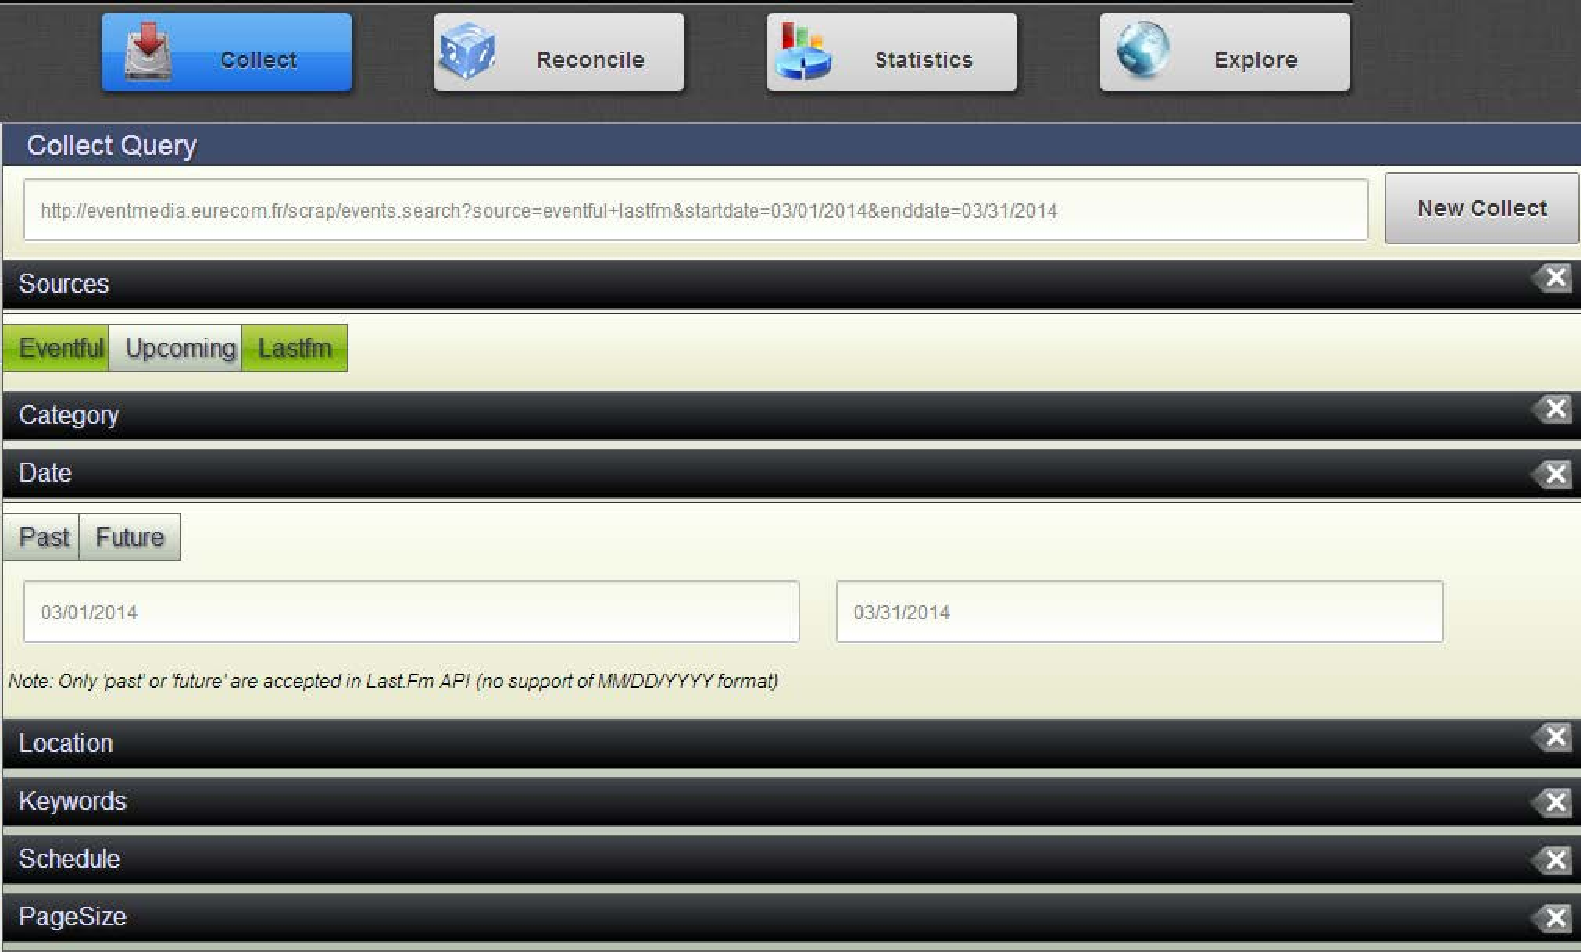
\includegraphics[width=\linewidth]{dashboard.pdf}
  \caption{Collect Events Mode - Building a query}
  \label{fig:dashboard}
\end{figure}

\begin{figure}[htbp]
  \centering
  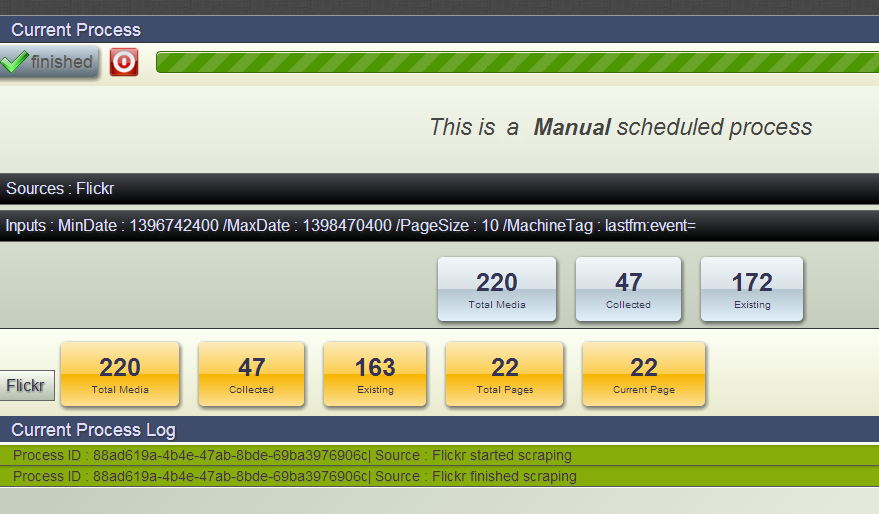
\includegraphics[width=\linewidth]{process-dashboard.png}
  \caption{Collect Media Mode - Monitoring Scraping Processes}
  \label{fig:process-dashboard}
\end{figure}

\begin{figure}[htbp]
  \centering
  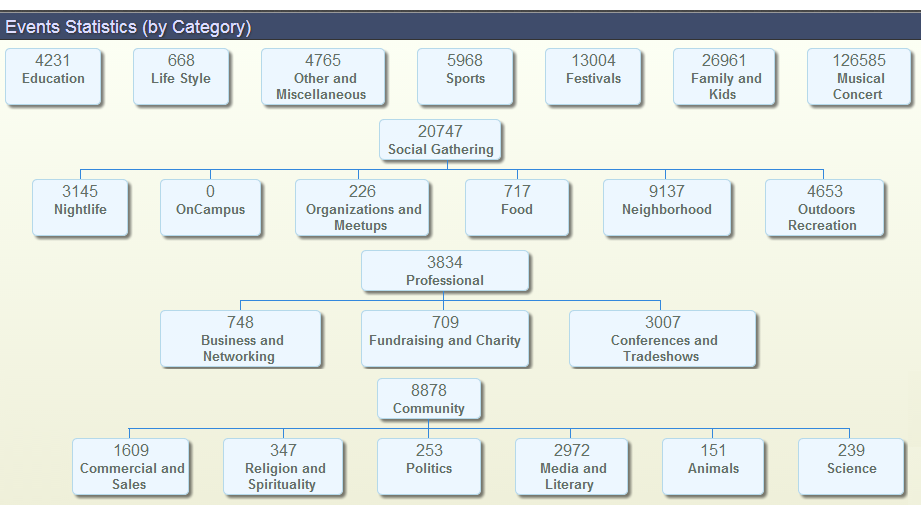
\includegraphics[width=\linewidth]{stats-dashboard.png}
  \caption{Statistics Mode -  Number of events per category}
  \label{fig:stats-dashboard}
\end{figure}

In order to ensure a permanent progress visualization of the scraping processes, a timer has been set to request the progress service of our framework and to update accordingly the dashboard (Figuree~\ref{fig:process-dashboard}). The same timer also updates the console log section by requesting the log service which provides status messages in different types (Debug, Warning, Error). Finally, the dashboard provides \textit{Statistics} view to show useful information about the dataset such as the number of collected instances per type. Figure~\ref{fig:stats-dashboard} depicts, for example, the number of events per each category. Technically, the languages used are HTML 5 and Javascript with the simple and powerful library jQuery UI. Google maps API and Charts were also used to provide data visualization on maps or to draw chart visualizations.

\section{Semantic Data Modeling}   \label{sec:data-modeling}
The motivation behind the use of Semantic Web technologies is their prominent success to provide a flexible support for large-scale data integration. Indeed, a long standing challenge in information systems is to integrate data from distributed, heterogeneous, and autonomous data sources. This refers to the problem of combining data spread across different sources, and providing the user with a unified view of these data. The crucial task lies in forming the relations between the heterogeneous data sources and a global schema representing the unified view. Data sources, some of them being available on the Web, are autonomously designed and operated. As a consequence, they use different systems (e.g. flat files, relational database), data models and access queries. Combining these distributed sources within one application needs an additional layer. This layer has to dynamically integrate data and facilitate interoperability between different structures. In the literature, several integration layers have been proposed as joint efforts of research communities from various fields such as Database, Artificial Intelligence and Semantic Web. One solution widely adopted in recent years is the use of ontologies, which is favored in various disciplines such as biology, medicine and e-government~\cite{Shadbolt:SWR06}. In the context of Web services, Szomszor et al.~\cite{Szomszor:CCGrid05} have shown the efficiency of ontology-based representation to achieve data harmonization when a mismatch in data formats occurs. The underlying goal of using ontology is to provide a conceptual model that can be shared by different applications. There is an emphasis on knowledge reuse and on the creation of common ontologies which can be extended for more specific applications. This has led to different vocabularies allow describing resources across various domains and facilitate semantic interoperability of metadata. In our case, we use ontologies to enable large-scale integration of data provided by event and media Web services. But, what vocabularies are suitable for representing relationships between events and related entities such as time, location, agent and media? 

Given the event definition introduced in Section~\ref{sec:events-def} and the intrinsic connection between events and media, we consider events as:

\begin{itemize}
\item A natural way for referring to any observable occurrence grouping persons, places, times and activities that can be described~\cite{Shaw:ASWC09}.
\item Observable experiences that are often documented by people through different media (e.g. videos, photos and tweets).
\end{itemize}

In order to formalize this definition, we propose the following ontological models that represent events as well as the related media.

\subsection{Event Modeling: the LODE Ontology}
To represent events, we use the LODE ontology\footnote{\url{http://linkedevents.org/ontology/}} which is a minimal model that encapsulates the most useful event properties~\cite{Shaw:ASWC09}. LODE complies with the event definition provided in Section~\ref{sec:events-def}. It is not yet another ``event'' ontology \emph{per se}. It has been designed as an \emph{interlingua} model that solves an interoperability problem by providing a set of axioms expressing mappings between existing event models. Hence, the ontology contains numerous OWL axioms stating classes and properties equivalence between event models such as EO~\cite{Raimond:ISMIR07}, CIDOC-CRM~\cite{Doerr:03} and ABC~\cite{Lagoze:DCMI01} to name a few. 

Overall, the goal of LODE is to enable an interoperable modeling of the ``factual'' aspects of events, where these can be characterized in terms of the four Ws: \emph{What} happened, \emph{Where} did it happen, \emph{When} did it happen, and \emph{Who} was involved. ``Factual'' relations within and among events are intended to represent intersubjective ``consensus reality'' and thus are not necessarily associated with a particular perspective or interpretation. We use the LODE ontology together with properties from FOAF~\cite{Foaf:2014}, Dublin Core~\cite{DublinCore:2012}, and vCard~\cite{vCard:2013}. Our strategy is to separate events from their interpretations with an emphasis on factual aspects, a design approach different from the other event models. 

Figure~\ref{fig:lode-ontology} depicts the LODE model of the event identified by \emph{ID=3163952} on Last.fm. More precisely, it indicates that an event categorized as a \texttt{Concert} has been given on the \texttt{21th of May 2012 at 12:45 PM} in \texttt{The Paramount Theater}, featuring the \texttt{Snow Patrol} rock band and having participant named \texttt{earthcapricor}. This event also exists in Upcoming directory but with another identifier \emph{ID=3163952}. To sum up, a graph representing an event contains the category of the event, a text description, a date (instant or interval represented with OWL Time~\cite{OwlTime:2013}),  a location in terms of geographical coordinates (latitude, longitude) and a URI of the venue, and finally the agents (e.g. artists) and attendees involved. A graph representing an agent is composed of a label, description (e.g. biography), tags and often a photo. A graph for location contains a label and different address fields (e.g. street , city, postal code, country). A graph describing a user contains a label, user's real name and often an avatar.

\begin{figure}[htb]
  \centering
  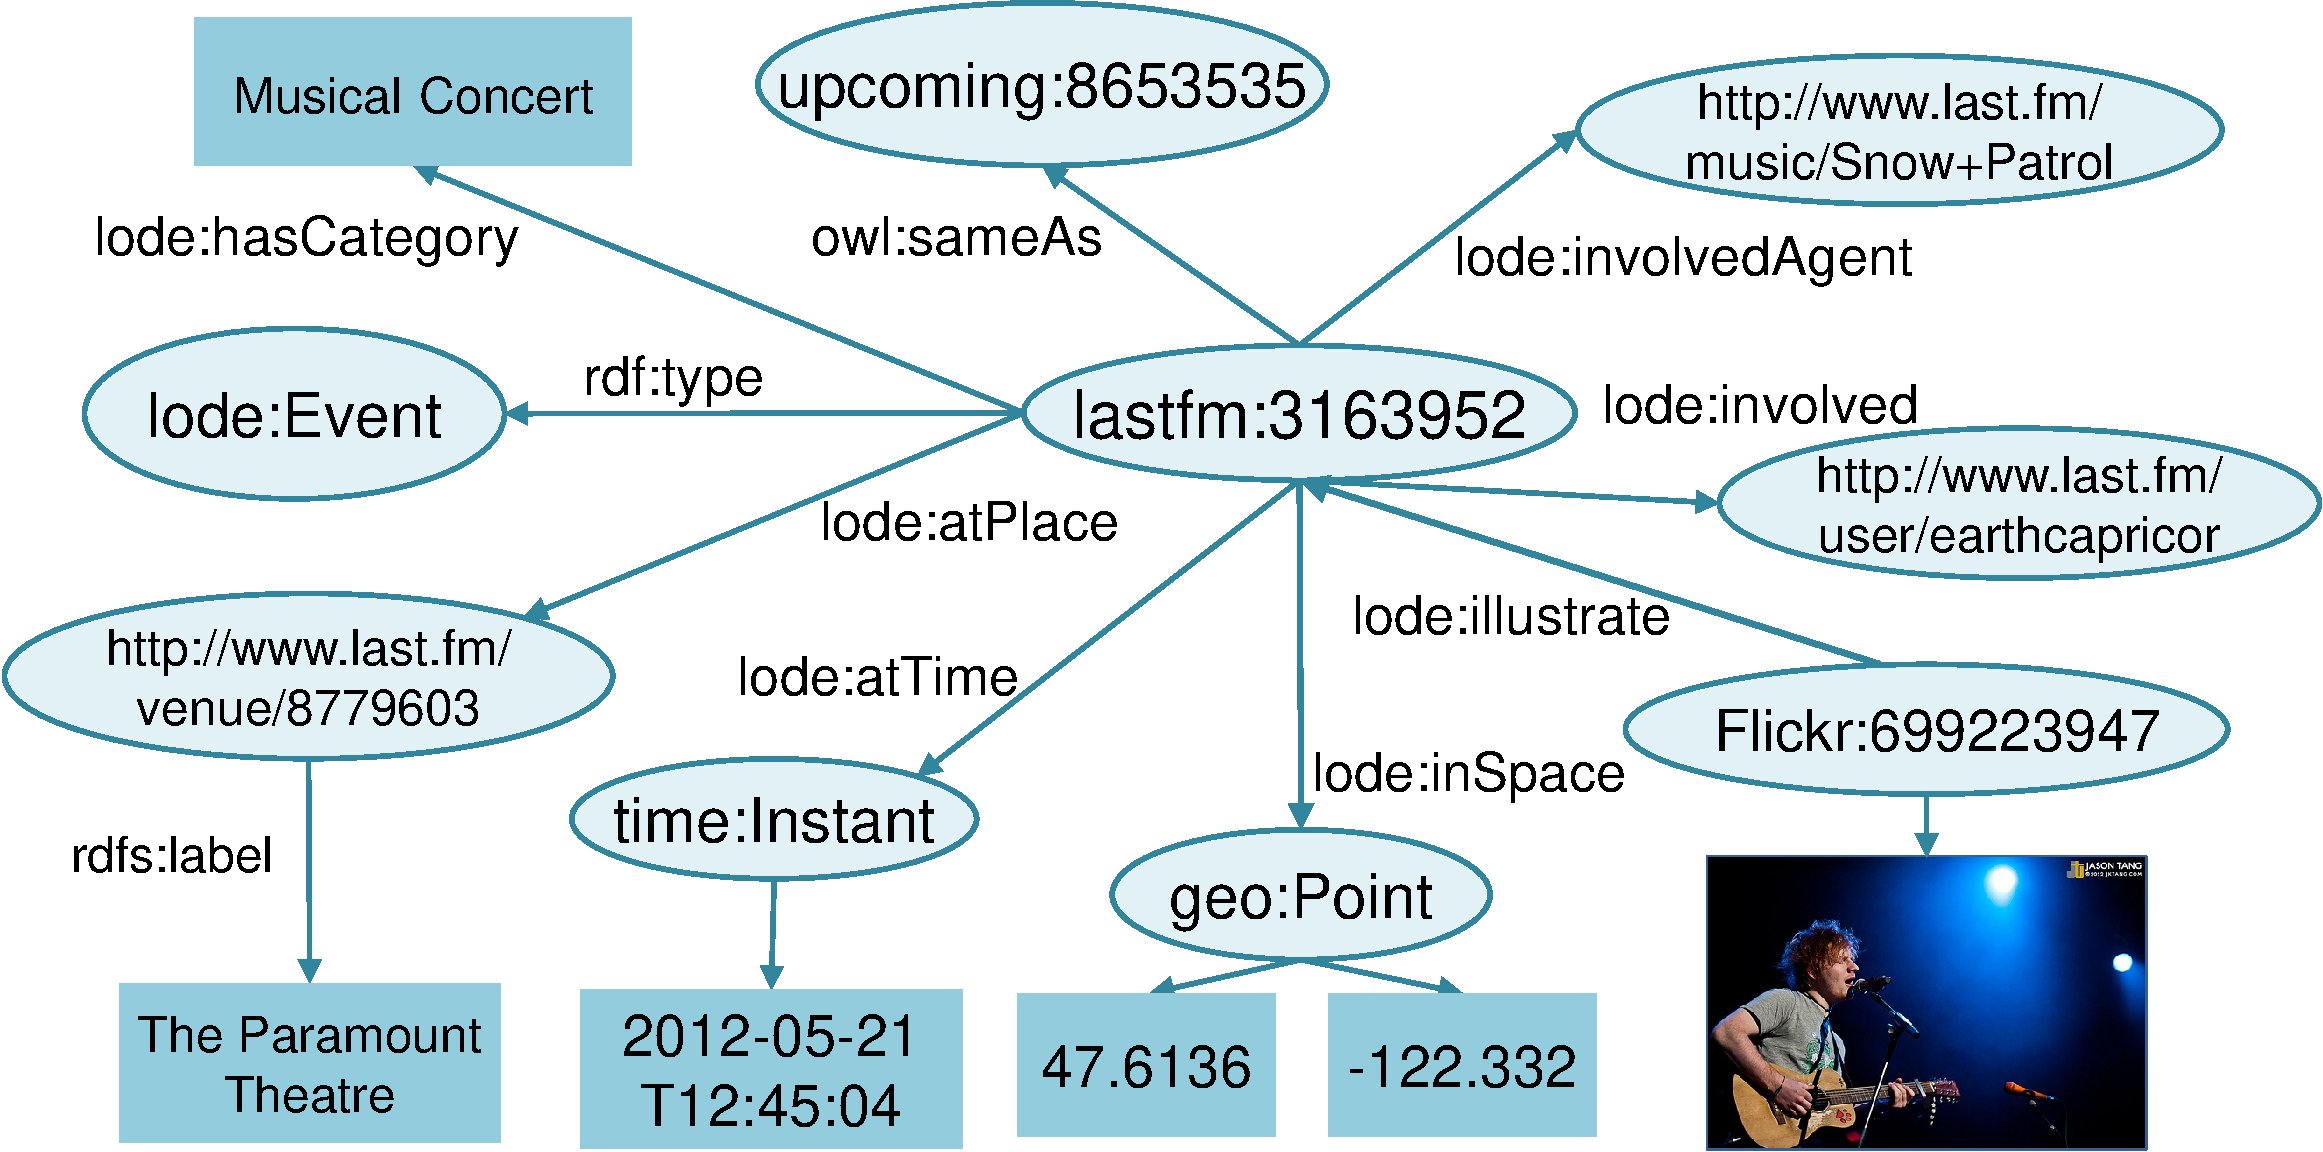
\includegraphics[width=\linewidth]{lode-ontology.pdf}
    \caption{The \emph{Snow Patrol Concert} described with LODE ontology}
  \label{fig:lode-ontology}
\end{figure}

Finally, we propose to organize events in a taxonomy that solves the interoperability of existing classifications. In general, events are categorized in lightweight taxonomies that provide facets when browsing event directories. We manually analyzed the event taxonomies used in various websites, namely Facebook, Eventful, Upcoming, LinkedIn\footnote{\url{http://www.linkedin.com}}, Eventbrite\footnote{\url{http://www.eventbrite.com}} and Ticketmaster\footnote{\url{http://www.ticketmaster.com}}, and we used card sorting techniques in order to build a rich SKOS thesaurus of event categories. SKOS~\cite{SKOS:2009} stands for Simple Knowledge Organization System. It provides a vocabulary to represent knowledge organization systems. Such representations include classification schemes, taxonomies and other structured controlled vocabularies. Our SKOS thesaurus contains axioms expressing mapping relationships between the different event taxonomies on the Web. The event taxonomy in our own namespace is accessible online at \url{http://data.linkedevents.org/category}. 

\subsection{Media Modeling}
In order to represent media, we use two popular vocabularies namely, the W3C Media Resource Ontology~\cite{MediaOnt:2009} and the SIOC vocabulary~\cite{SIOC:2010}. The link between events and media is realized through the \texttt{lode:illustrate} property. 

The Media Resource ontology is a W3C initiative that defines a core vocabulary to cover most commonly used annotation properties of media resources (e.g. image, audio, video). Such properties include different types of metadata such as locator, creation date, genre, rating, thumbnails, among others. Media fragments can also be defined to have a smaller granularity and attach keywords or formal annotations to parts of a media item. The ontology contains a formal set of axioms to define the mapping between different metadata formats for multimedia. We use this ontology together with properties from SIOC, FOAF and Dublin Core to convert into RDF the description of Flickr photo (figure~\ref{fig:flickr-model}) and YouTube video. More information can be attached to the URI of the photo or video creator having \texttt{sioc:UserAccount} as RDF type.
 
\begin{figure}[htb]
  \centering
  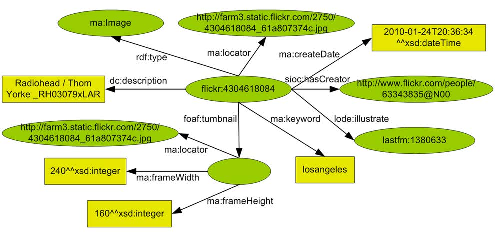
\includegraphics[width=\linewidth]{flickr_radiohead.pdf}
  \caption{A photo taken at the \emph{Radiohead Haiti Relief Concert} described with the Media Ontology}
  \label{fig:flickr-model}
\end{figure}

\begin{figure}[htb]
  \centering
  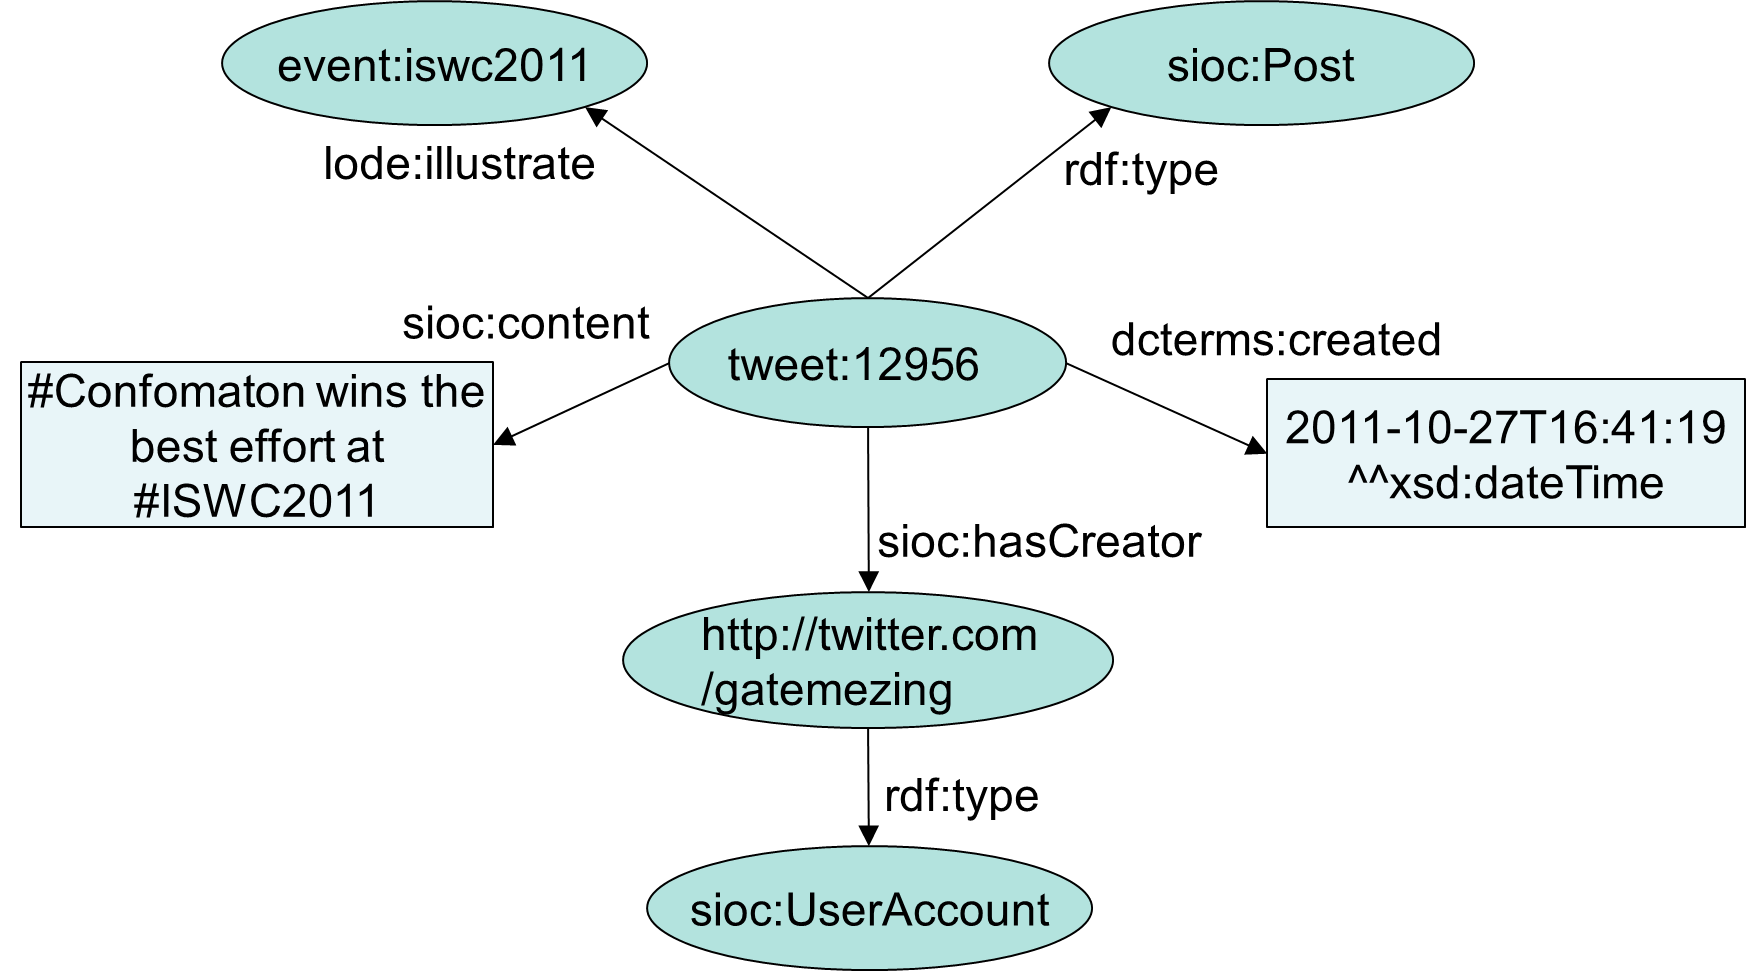
\includegraphics[scale=0.43]{sioc.png}
  \caption{RDF modeling of microposts using the SIOC Ontology}
  \label{fig:sioc-model}
\end{figure}

SIOC stands for Semantically-Interlinked Online Communities. It provides a core ontology about the main concepts required to describe information about online communities (e.g. wikis, blogs). Such information can include post title, author, keywords, date or the full post text in community sites. SIOC becomes a standard way to model the underlying structure of the user-generated content from social media sites. We use it together with Dublin Core properties to convert into RDF the description of microposts (Figure~\ref{fig:sioc-model}).

\vspace*{2mm}
%%%%%%%%%%%%%%%%%%%%%%%%%%%%%%%
%%%  4. EventMedia Dataset  %%%
%%%%%%%%%%%%%%%%%%%%%%%%%%%%%%%
\section{EventMedia Dataset}		\label{sec:eventmedia-dataset}

The so-called EventMedia dataset contains data that we collected from four public event directories (Last.fm, Eventful, Upcoming and Lanyrd), and from three public media directories (Flickr, Youtube, Twitter)~\cite{Khrouf:SWJ12}. It consists of more than 30 millions RDF triples providing descriptions of events and related media based on LODE, Media Resource and SIOC ontologies. EventMedia is a hub in the Linked Data cloud since September 2010. We mint new URIs into our own namespace such as for
events\nofootnote{\url{http://data.linkedevents.org/event/}} and
agents\nofootnote{\url{http://data.linkedevents.org/agent/}}. All URIs are dereferencable and served as static RDF files serialized in many formats such as RDF/XML, N3 and N-Triples. They are also accessible using a SPARQL endpoint\footnote{\url{http://eventmedia.eurecom.fr/sparql}} and a RESTful API\footnote{\url{http://eventmedia.eurecom.fr/rest/{resourceId}}} powered by the Linked Data API (detailed in Section~\ref{sec:elda}). Table~\ref{tab:dataset-stats} provides an overview about the number of resources per type and source, and Figure~\ref{fig:eventmedia-dataset} illustrates the main components of EventMedia.

\begin{table}[H]
\centering{
\begin{tabular*}{13.5cm}{l| @{\extracolsep{\fill}} c|ccccc}
\hline
 &  & \textbf{Event}  & \textbf{Agent} &  \textbf{Location}& \textbf{Media} & \textbf{User}  \\
\hline
\multirow{4}{*}{Event Sites} &

 Last.fm & 69,185   & 81,006  & 18,653  & 7,795 & 213,351 \\ 

&  Upcoming  & 29,418  &      78   &  14,372  &   29 &  23,977 \\

&  Eventful  & 84,225   &   11,226  & 30,572 &      15,532  &     547 \\

& Lanyrd    & 2,151   &   	-  &    624  &     -  &      - \\    
  \hline
  \hline
\multirow{2}{*}{Media Sites} & 
Flickr    & -   &   	-  &    -  &    1,879,343 &      25,219 \\ 
& Youtube    & -   &   	-  &    -  &     517  &      - \\
& Twitter    & -   &   	-  &    -  &     1,060,879 &      267,138\\
  \hline
\end{tabular*}
\caption{Number of different resources in EventMedia dataset per type and source}
\label{tab:dataset-stats}
}
\end{table}

\begin{figure}[H]
  \centering
  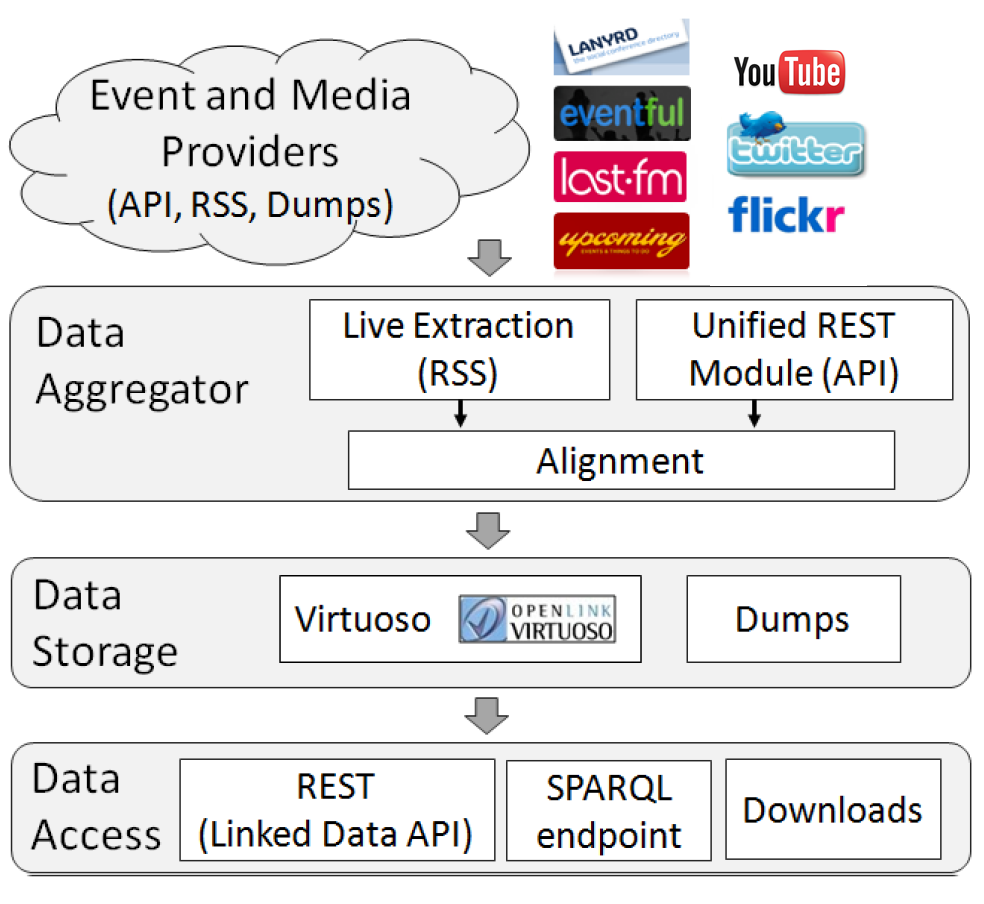
\includegraphics[scale=0.34]{eventmedia-dataset.png}
  \caption{Overview of the EventMedia components}
  \label{fig:eventmedia-dataset}
\end{figure}


\section{Conclusion}   \label{sec:conclusion}
In this chapter, we described our framework designed to aggregate data with the aim to ensure a certain level of flexibility. We also exploited the Semantic Web technologies to integrate at large scale the information contained in event and media directories. As for the semantic modeling, our design is based on the LODE, Media Resource and SIOC ontologies used to describe events and different types of media (e.g. photo, video, micropost). Data collected is converted to RDF and then stored in EventMedia dataset. Ultimately, we aim at providing an event-based environment to deliver enriched views and enhance the event discovery.

